\chapter{Nubby's Girlfriend}

\begin{wrapfigure}{O}{\figwidth}
	\begin{center}
		
\includegraphics[width=\figwidth]{pics/5/1.png}
	\end{center}
\end{wrapfigure}
The squad is currently staring goggle-eyed at their Interrogator, who just so happens to be the most beautiful woman they have ever seen. 
They have just boarded the shuttle to their next mission, which they are being informed, involves purging multiple genestealer cults from an imperial world. 

Doc is stuttering out a few poorly worded questions and trying not to stare at the Interrogator’s chest while Cutter has already wandered off and is playing with his chainsword. 
Twitch and Nubby both tried to run for the exit at the world ‘genestealer’ and only Sarge’s iron grip is holding them back. 
Behind the Interrogator there are five professional looking men who are eyeing the guardsmen with dubious expressions.

\begin{wrapfigure}{O}{\figwidth}
	\begin{center}
		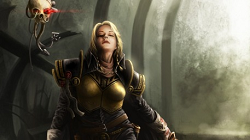
\includegraphics[width=\figwidth]{pics/5/2.png}
	\end{center}
\end{wrapfigure}
So no shit there we were, heading out to fight the foes of the Imperium under to command of the hottest woman within several cubic light years. 
Sure we were on our way to fight with a bunch of xenos monstrosities and mutant cultists, but our Interrogator was the envy of inquisition agents all across the sector. 
Any red blooded trooper would have given his right hand to trade places with us, except he’d need it for the long lonely nights after she’d ruined every other woman for him. 

None of us had imagined there was ever an Interrogator like her, she was practically perfect. 
She had a dancer’s grace, a charmer’s smile, and a singer’s voice; everything about her was beautiful and perfect. 
To top it all off she had experience running every part of an inquisition operation, was a minor psyker, and was absolutely deadly with her force sword. 
It was a wonder that she wasn’t already an Inquisitor, we all assumed that her boss had just wanted to keep her around as long as possible.

The rest of the team consisted of hard bitten multi-discipline adepts that could only really be called agents. 
They each had a bit of a specialty, such as technology or stealth or social infiltration, but they were all highly trained operatives that could fill almost any role in a mission. 
On top of that, every single one of them was wrapped around our Interrogator’s little finger, they’d go into the eye of terror itself if she ordered it. 
They hung on her words at briefings and were constantly researching and practicing in hope of earning her praise. 

So it was sort of surprising that most of us didn’t really like her.

\begin{wrapfigure}{O}{\figwidth}
	\begin{center}
		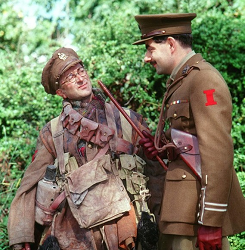
\includegraphics[width=\figwidth]{pics/5/3.png}
	\end{center}
\end{wrapfigure}
Doc and Twitch were terrified of her. Doc got tongue tied around most women, he could barely even talk when the Interrogator was around. 
He would drop what he was holding, stare at anything else in the room, then either freeze completely or mutter something and try to escape. 
Meanwhile Twitch had decided that anything that beautiful was specifically designed to destroy men.
He firmly believed that she was some sort of daemon, or witch, or xenos, or mechanical construct; 
his theory varied from day to day. Their relationship was not helped by her repeated insistence that he not wire everyone’s quarters with mines.

Sarge and Cutter were vaguely distrustful of her. Sarge had a completely justified distrust of authority: 
none of the squad’s previous Interrogators had impressed him with their strategic ability and his guard superiors had been even worse. 
On top of this, while she was easier on the eyes than any of his former bosses, Sarge automatically assumed that any superior officer that didn’t have at least one obvious battle wound probably spent most of their time getting guardsmen shot instead. 
For his part, Cutter didn’t understand what all the fuss was about. 
Sure the Interrogator’s force weapon was pretty cool, but there was only room in his heart for his chainsword-chan.

Nubby immediately fell in love though. He followed the Interrogator around like a foul mouthed, unhygienic, kleptomaniacal puppy.

\begin{wrapfigure}{O}{\figwidth}
	\begin{center}
		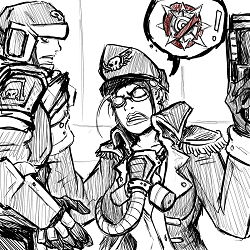
\includegraphics[width=\figwidth]{pics/5/4.png}
	\end{center}
\end{wrapfigure}
Honestly we weren’t sure who we felt more sorry for. 
Nubby’s constant attempts to impress her were absolutely pathetic, but on the other hand she had to endure Nubby’s near constant presence. 
He would follow her around doing errands, offering her little gifts, and constantly telling her about the heroic exploits of Captain Nubby and his merry men. 
At first she encouraged this behavior, since Nubby was the only man in our squad that would give her anything more than a resigned salute. 
Everyone has their limits though and Nubby’s chatter, blatant thievery, and SMELL could wear down anyone’s patience. 
He even started standing guard outside her quarters while she slept, which was more than anyone should have to bear. 
Sarge put a stop to that as a sort of peace offering. 

Once again, we claimed a section of cabins as our own and let Twitch fortify them. 
Thanks to our abysmal first impression, not to mention effect Nubby had on the rest of the team, we mostly got away with our routine of napping, PT, and ignoring everyone else. 
The others seemed to think of us as disposable muscle, and they definitely weren’t about to traverse a literal mine-field or argue with a heavily armed paranoid just to talk to us. 
Of course we had to leave our territory to go to a few briefings with the rest of the team, but since we weren’t part of the Interrogator Fan Club we weren’t invited to stick around in their part of the ship. 
The only exception to our isolation was that every once in a while the Interrogator would come down and make an attempt at bonding with us. 
She stopped trying after Twitch threw holy water at her though.

The end result of all this mutual disgust, aside from making any casual conversation with Nubby unbearable, was that Nubby more or less became the liaison between our squad and the rest of the team. 
This meant that almost all the information about our mission went through a pathological liar who spent most of the time making eyes at the Interrogator instead of listening.

\begin{wrapfigure}{O}{\figwidth}
	\begin{center}
		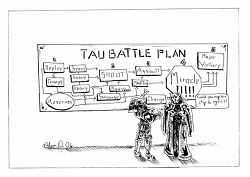
\includegraphics[width=\figwidth]{pics/5/5.png}
	\end{center}
\end{wrapfigure}
The information that filtered through to us wasn’t exactly encouraging. 
A major genestealer cult had been broken up several years ago by some badass Inquisitor, but several splinters had already broken off and headed for other worlds. 
Recently several of those splinters had been tracked down to a medium sized imperial world smack in the middle of the sub sector. 
Oak had apparently decided that this was an excellent chance for some of the Inquisitor wannabes to prove themselves, so three teams were sent out to try and purge these infestations WITHOUT massacring entire Imperial cities. 
A few regiments of guard would be stopping by in a few months, so if the teams failed to solve things by then a more general purge would be performed by the boys in green.

Our three team force was given the rough location of no less than six genestealer infestations and told to go down and pinpoint each cult, take out its leadership, and then send in the locals to mop up the rest. 
Everyone would enter the system discreetly, so as not to spook the cults, and each Interrogator was given a trainee rosette to beat the local authorities over the head with. 
Each team was assigned two infestations and told to help the others when they finished or if the other teams called for help. 
Finally, if shit went south they were to try and convince the PDF to do a general purge. % TYPO puge to purge

Our Interrogator and the Agents spent the trip going going through what info we had about the planet and the cults. 
The general theory was to find the public face of the cults, perform some sort of daring kidnapping operation, rip the location of the rest of the cult from their minds or databases, then plan a surgical strike with loyal elements of the PDF. 
We all eagerly awaited the second plan that would be formed after the attempt to capture a psychotic, mutant, xenos cultist surrounded by guards went ploin shaped.

\begin{wrapfigure}{O}{\figwidth}
	\begin{center}
		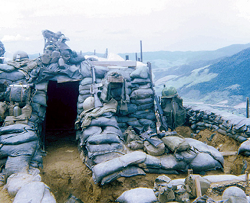
\includegraphics[width=\figwidth]{pics/5/6.png}
	\end{center}
\end{wrapfigure}
We touched down in a fair sized city and immediately set up base in a pretty ritzy house, apparently the Inquisition wasn’t skimping on this mission. 
The agents all started going out on their little fact finding missions: 
infiltrating political groups, examining real estate records, hacking databases, and in the Interrogator’s case, attending extravagant parties. 
We were not invited on any of these missions on the grounds that we were so unstealthy that just being in the same general area would blow their cover. 
The lack of invitation didn’t stop Nubby from attending the parties though, one can only imagine the disgust on the Interrogator’s face when he kept showing up mid party in clothes he’d mugged off a servant or drunk nob.

Since we didn’t have anything better to do we mostly lounged around, ate bad fast food, kept the vehicles in order, and generally transformed a beautiful town house into an Imperial Guard firebase. 
We had been in transit for several weeks and now we had been told to stay at base while the rest of the team did the investigating. 
While any guardsman appreciates down time, Sarge wasn’t a fan of troopers sitting around with nothing to do, so he stepped up the schedule of our drills and we all helped Twitch fortify the place. 
This eventually got us in trouble with the Interrogator, since apparently surrounding a house with razorwire counts as breaking cover, even if you cover it up with decorative shrubbery.

\begin{wrapfigure}{O}{\figwidth}
	\begin{center}
		
\includegraphics[width=\figwidth]{pics/5/7.png}
	\end{center}
\end{wrapfigure}
Our relationship with the rest of the team was definitely getting a bit strained. Cutter got yelled at for doing sword drills in the middle of the night:
apparently some of the agents had trouble sleeping while someone was revving a chainsword and screaming obscenities at a training servitor. 
They were also unappreciative of Sarge holding 5am PT in the back yard, and Doc’s insistence that everyone submit to a thorough physical. 
The real problems were Twitch and Nubby though.

Of course Twitch was doing his usual thing, but unlike our previous teams the agents had no appreciation for a properly secured perimeter. 
After an Agent ignored the posted directions and had to be rescued from a depressed land mine there was a big fight between Twitch and the Interrogator. 
His perfectly valid points about perimeter security, posted instructions, and the relative safety of mechanical dual action mines compared to motion activated ones were dismissed; 
in the end he had to remove all booby traps outside the squad’s quarters, even the non-lethal ones.

To top everything off Nubby had ground the entire team’s nerves down to the bone. 
His constant petty theft, chatter, and poor hygiene were bad enough, but he was practically stalking the Interrogator at this point. 
His very presence offended the Agents, and his behavior drove them all into a simmering rage. 
Only his fictitious rank of Captain and supposed command of our squad kept them from killing him or banning him from their briefings.

All in all it was a relief for everyone when they finally identified the front for the local cult and their primary moles in the local government.

\begin{wrapfigure}{O}{\figwidth}
	\begin{center}
		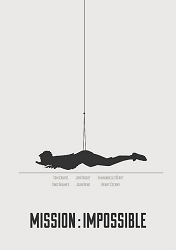
\includegraphics[width=\figwidth]{pics/5/8.png}
	\end{center}
\end{wrapfigure}
The plan our Interrogator came up with was a beautifully choreographed series of misdirections and lightning strikes. 
There were cunning disguises, perfectly placed bribes, subtle pieces of blackmail, nearly impossible feats of stealth and speed, and in the middle of it all would be our Interrogator acting as the maestro. 
Every agent would work in perfect sync to draw the targets in, subdue them, and then return them with their memories modified and the cult none the wiser. 
Our squad would stay in the van and do absolutely nothing to screw things up.

An extravagant party was organized by the Interrogator and every one of the targets received an invitation they couldn’t possibly refuse. 
A venue was chosen, disguises were perfected, traps were set, and a little out of the way room was filled with several sinister pieces of equipment and a very nervous Doc. 
Doc was the only one allowed to even enter the building during the operation, and that was only because no one else was qualified to handle anesthesia. 
Mind you Doc wasn’t really qualified either, his past experience with sedation primarily consisted of sticking unhappy people with the guard-issue one use morphine amps.

The plan called for a lot of really complex stuff that more or less boiled down to grab a target, take them to the little room, drug them, do psyker stuff to them, dump them back in the party with a gap in their memory, then repeat. 
Cynics that we were, we fully expected this to fail horribly. 
Our squad sat in the van armed to the teeth, listening to the comms, and just waiting for the screaming to start.

It was a bit of a let down when things went off without a hitch.

\begin{wrapfigure}{O}{\figwidth}
	\begin{center}
		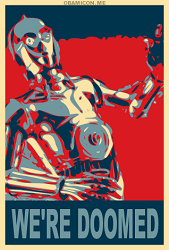
\includegraphics[width=\figwidth]{pics/5/9.png}
	\end{center}
\end{wrapfigure}
The social agents socialed, the stealthy agents stealthed, the psyker agent psyked. 
One after another the targets were brought to Doc’s little room where he kept them sedated while  our Interrogator and her assistant rooted around in their deformed brains. 
The closest thing to a problem was when Doc found out that a genestealer hybrid is rather resistant to most tranquilizers, but immediately quintupling the dosage solved that problem. 
In a remarkably short amount of time we had all the information we needed on the local cult, and the victims had no idea that anything had happened. 
We were absolutely floored.

Seriously, the mission had taken less than an hour from the word go. 
Most of the night was taken up with going through the motions of the party while our squad sat in the van like a bunch of naughty children. 
It was the most successful Inquisitorial op we’d seen and Nubby gave us no end of shit about doubting his girlfriend. 
He was so goddamn insufferable that we eventually kicked him out of the van and told him to go stalk the Interrogator or something for the rest of the night.

The data gained from the party was used to create a detailed list of targets for surgical strikes by the local authorities. 
The list was packaged with several strategic ‘suggestions’ and dire warnings about the consequences of failure, then sealed by the Interrogator and handed off to a few powerful local officials who were believed to be trustworthy. 
We got to come along and watch as these packages were delivered, the snooty bastards nearly shit themselves when they were shown the Interrogator’s Rosette. 

The Interrogator sealed the packages and instructed the locals to only open them if ordered to do so by someone with an Inquisitorial Rosette. 
That done, we all packed up, sent a coded message to the other teams informing them of our success, and headed for the next cult location.

A less stalwart bunch of guardsmen would have started to doubt their cynical view of the world, but we had earned every bit of that cynicism with blood, sweat, and tears. 
Like hell were we going to give it up for something as trifling as a single successful mission. 
We comforted ourselves with the thought that nothing that perfect could happen twice. 
We told ourselves that the next op was practically guaranteed to have a colossal fuckup in it, even if we had to supply it ourselves.

Boy were we right.

\begin{wrapfigure}{O}{\figwidth}
	\begin{center}
		
\includegraphics[width=\figwidth]{pics/5/10.png}
	\end{center}
\end{wrapfigure}
We moved to another of the major cities on the planet and once again we set up shop in an incredibly posh house. 
We went about guardifying it while the rest of the team did their intel gathering things, but we were much more restrained this time. 
The success of the previous mission had been humbling. 
The team had put up with our shit and performed like professionals; the least we could do was be civil. 
That’s not to say that we were any more fond of the Interrogator or any less sure of the impending disaster, we just didn’t see the point of deliberately pissing the rest of the team off while they worked. 

Even though we were acting more retrained our paranoia had been ratcheted up several levels by the success, it was just a morose sort of paranoia. 
Something was inevitably going to go wrong, but no one would ever listen to us or let us take perfectly reasonable security measures. 
So we just stewed in our makeshift barracks and prepared for all the complex plans to fall apart and dump everything into our laps. 
Our mood was not improved by Nubby periodically coming in and rambling about his lady love.

\begin{wrapfigure}{O}{\figwidth}
	\begin{center}
		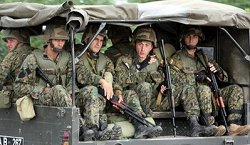
\includegraphics[width=\figwidth]{pics/5/11.png}
	\end{center}
\end{wrapfigure}
Before long the intel was gathered, the targets were identified, and another magnificent party was scheduled by the Interrogator.
Once again the Interrogator and her agents put together an incredibly complex plan which would pull one target after another into the little interrogation room manned by Doc. 
There were little differences here and there, but it really was the same plan as last time. 
Right down to us grumpy guardsmen sitting in the van where couldn’t get into trouble.

We paid careful attention to the briefing this time, quietly tracking all the ways things could go wrong. 
When it was over we retreated to our quarters and started making our own contingencies. 
We had plans for stopping escaping targets, we had plans for intercepting cultists hunting our team, we had plans for holding off reinforcements. 
Hell, we even had plans for if the Interrogator and the psyker agent both simultaneously turned into daemonhosts. 
Sure all these plans were more or less “apply las fire and explosives until it stops being a problem,” but we did have them.

The team was amped up and ready for another perfect op. 
Well at least Nubby, the agents, and the Interrogator were, but after several days of morosely speculating about what would go wrong our squad had the general attitude of condemned prisoners. 
We weren’t sure what would be worse; 
if even a tenth of our paranoid worries came true we were all going to die horribly, but if everything went perfectly again we’d probably have to kill ourselves or join the Interrogator Fan Club with Nubby. 
Most of us considered death to be the better option.

\begin{wrapfigure}{O}{\figwidth}
	\begin{center}
		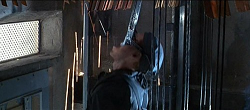
\includegraphics[width=\figwidth]{pics/5/12.png}
	\end{center}
\end{wrapfigure}
On the night of the party our squad piled into the van with so much military hardware that we clinked when we walked. 
We had lasguns and melee weapons, ammo and medpacks, several different types of grenades, and more detpacks than even Twitch thought we needed. 
When a guardsman feels a sense of doom in the air, munitions are his security blanket.

Doc was sent off to his little room with a batch of super heavy tranquilizers he had prepped after the slight difficulty last time. 
He was going to be alone in there so we gave him a backup guard issue combead and, in direct violation of the Interrogator’s orders, Twitch snuck him a few of his toys. 
That is to say, Doc was given enough directional mines to blow anyone coming through the front door to chunky salsa while simultaneously opening an escape route out the back.

We sat in the van, jittering and waiting for either the impending disaster or the most embarrassing moment of our lives. 
This op would make us, break us, or quite possibly kill us; all we could do was listen to the comms and wait to see which. 
You should have seen the look on Sarge’s face when the elevator the stealthy agent was on suddenly reversed direction and smashed him into the top of the shaft.

\begin{wrapfigure}{O}{\figwidth}
	\begin{center}
		
\includegraphics[width=\figwidth]{pics/5/13.png}
	\end{center}
\end{wrapfigure}
Grinning like schoolboys, we started piling out of the van even before the agent’s scream was cut short by the inevitable *splat*. 
As we sprinted for the building we all felt a deep sense of satisfaction as two of the agents reported they were being followed, and Sarge almost started laughing when the Interrogator’s order to abort was interrupted by a gurgling scream and comms going down. 
Twitch actually did start laughing when Doc reported hostiles approaching his position and his intention to blow the mines then rendezvous with us in the ballroom.

We hit the front doors right as Doc’s mines went off. 
As the explosion shook the building we kicked in the door, buttstroked the rent-a-cops standing guard, and headed for firing positions. 
Nubby and Twitch sprinted up into the balconies to lay down covering fire while Sarge and Cutter started forcing a path through through the crowd. 
It was complete pandemonium in the ballroom: 
the crowd was panicking, gunfire was coming from several directions, and the hostiles were almost identical to the rest of the party goers.

One agent was already down, another was pinned behind some pillars, and as we got into position we saw the Interrogator retreat out a side door with three cultists in pursuit. 
Nubby and Twitch made quick work of the cultists they could see and started sweeping the crowd for hostiles and the original targets. 
Sarge and Cutter finally made it through the crowd to the surviving agent where they found several cultists pretending to be guests and waiting for a clear shot.
Cutter hit them in the rear and started making cultist hamburger while Twitch and Nubby shot anyone who didn’t run from the madman with a sword. 
Sarge took this chance to run in and grab the pinned agent before more hostiles showed up.

The ground team was pulling back towards the front doors when the rescued agent spotted one of the targets in the dwindling crowd and broke away from the group.

\begin{wrapfigure}{O}{\figwidth}
	\begin{center}
		
\includegraphics[width=\figwidth]{pics/5/14.png}
	\end{center}
\end{wrapfigure}
Swearing under their breaths Sarge and Cutter ran after the agent as he closed on a spectacularly fat man. 
The panic in the room covered the sound of the agent’s approach and he managed to land a decent hit with his stunner, but the fat man wasn’t completely incapacitated. 
With startling speed he popped back onto his feet, locked eyes with the agent, and started to draw a weapon. 
Before he could kill the paralyzed agent Cutter hit him like a truck and started repeatedly clubbing him over the head with the flat of his chainsword. 

Once the fat man stopped moving Sarge pulled Cutter off and the whole group headed for the exit dragging the fat man behind them. 
Twitch saw the cultists’ follow-up assassins enter the room before anyone else and immediately nailed two of them, prompting the rest to dive into cover. 
Thinking fast Sarge took cover behind the wobbling folds of the incapacitated target, and dragged Cutter and the agent down with him. 
They hunkered down behind the makeshift barricade and hoped to the Emperor that two hundred kilos of blubber would stop small arms fire.

It turned out that enough fat is just as good as a bunch of sandbags, and luckily the cultist’s didn’t have anything heavier than handguns. 
Twitch and Nubby picked off most of the cultists, and the last few decided to stick in cover and wait for reinforcements. 
Sarge was considered releasing Cutter to launch a flanking attack on them when Doc poked his head through the door behind the cultists.

\begin{wrapfigure}{O}{\figwidth}
	\begin{center}
		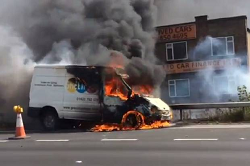
\includegraphics[width=\figwidth]{pics/5/15.png}
	\end{center}
\end{wrapfigure}
Doc ducked back out of the room and we all did our best to keep attention off of him for a few seconds. 
Before long he stepped out of the door, calmly walked up to a pair of cultists and tranqued them while behind him the last missing agent walked in and headshotted the final cultist. 
The room was empty except for us now, so Twitch and Nubby dropped down from the balcony and everyone gathered together to plan the next move.

The fat man was thoroughly dead; it turns out that no amount of body mass will let you live through being used as meat shield against half a dozen handguns. 
To our surprise the two cultists that Doc had so thoughtfully tranqued were dead too. 
Apparently they weren’t as genestealery as the previous targets had been and the quintuple strength tranq had instantly killed them. 
In fact a quick examination didn’t turn up anything genestealery about them. 
We had a vague feeling that this was important, but since it wouldn’t help us survive the current shitstorm we filed it away for later. 
Since we were the ones with working comms Sarge took operational command. 
The two surviving agents were told to fall in behind us, and we made our way out of the building.

Theoretically we should have tried to find the rest of the team first, but we knew one agent was dead and judging by the comm traffic the others were too. 
Nubby and the surviving agents argued for finding the Interrogator, but Sarge decided she was a big girl who could handle herself, so we all headed for base instead. 
We carefully made our way to the front door, and got ready for the completely exposed sprint to the van. 
Right as Sarge was about to give the order to run, the van exploded in a fireball that took out every other vehicle in the lot.

We all looked at Twitch, who shrugged and muttered about making sure no one tampered with it.

\begin{wrapfigure}{O}{\figwidth}
	\begin{center}
		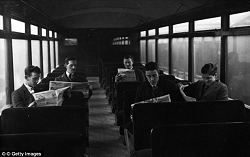
\includegraphics[width=\figwidth]{pics/5/16.png}
	\end{center}
\end{wrapfigure}
So no shit there we were, standing outside a building full of corpses (most of which WE were responsible for) with no vehicle, no form of Inquisitorial identification, and the rapidly approaching sound of sirens. 
Judging by the arm that landed next to Doc a bunch of cultists had tried to mess with our van and ran afoul of Twitch’s perimeter defenses, but no one shot the agents when we sent them to check on the wreckage so we assumed that none of the hostiles were left. 
We could have hotwired a nearby vehicle and lead the cops on a daring chase, or we could have had the social agent try to bluff them, or we could have silently gone into custody and awaited rescue by the Interrogator, or we could have even tried to fight our way through an entire city’s worth of cops. 
Instead we decided to just walk home.

The agents weren’t exactly happy about this decision; 
none of us were disguised they said, it was a twenty kilometer walk they said, we were in plain sight they said, and we were all obviously carrying weapons they said. 
We ignored them though, and as we walked Sarge calmly explained that no sane copper was going to ask a bunch of guardsmen why they were carrying their weapons with them on leave, especially not when there was something much more important to deal with. 
He did acknowledge the point about it being twenty klicks back to base though, so after a few blocks we found a train station and rode home with some very scared looking administratum workers. 
Those of us with proper Guard-issue common sense caught some much needed rest while we travelled, the agents just sat there and worried about their precious Interrogator.

The sun was almost up when we got back to base, and the agents were dead on their feet. 
Doc opened the front door and nearly lost a hand when the Interrogator fired several bolt rounds through it, but after a bit of careful negotiation we convinced her to let us in. 
She seemed surprised that we survived. It was a bit insulting really.

\begin{wrapfigure}{O}{\figwidth}
	\begin{center}
		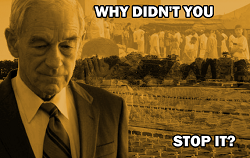
\includegraphics[width=\figwidth]{pics/5/17.png}
	\end{center}
\end{wrapfigure}
After the Interrogator put the bolt pistol down, we all filed in and Sarge gave the squad’s report. 
Doc and the agents filled in the bits he wasn’t there for, and we painted a pretty clear picture of the cultists’ attack, our swift response, and the rescue of the agents. 
Sarge also made sure to mention the attempt to capture the fat man and the lack of genestealer characteristics on the cultists, but the Interrogator wasn’t exactly impressed with this information. 
Instead she asked some very pointed questions about why the interrogation room had been filled with explosives, why we had deployed without orders, and whose idea it was to rig the van with proximity mines. 
For the most part we stood there and ignored these questions in traditional guardsman fashion, but Twitch made a few unkind comments about the Interrogator’s retreat which she graciously decided to ignore.

Eventually the Interrogator got tired of yelling at us and told the whole team to pack their gear up and get into the flier in the garage. 
She had decided that this part of the mission was beyond salvage and ordered an immediate purge by the PDF. 
We had less than an hour to get our shit together and get the hell out of there before the killing started. 

None of us were happy about the purge order. 
A whole lot of civvies were going to be killed and the PDF grunts were going to be pretty messed up by the end of the purge, but in the end, it was the Interrogator’s call to make. 
We didn’t have any clever suggestions and she clearly wasn’t interested in listening to our half-baked plans, so we kept our mouths shut. 
Hell, even if we had a real idea for fixing the situation we couldn’t have stopped the purge without the Interrogator’s Rosette.

So feeling like our heroic rescue had been for nothing, we collected everything we could carry, got into the team’s flier, and awaited further orders.

\begin{wrapfigure}{O}{\figwidth}
	\begin{center}
		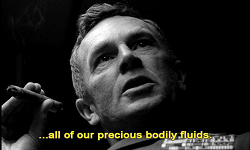
\includegraphics[width=\figwidth]{pics/5/18.png}
	\end{center}
\end{wrapfigure}
We hadn’t even finished stowing our gear when the Interrogator and the two agents sprinted into the flier in full combat gear. 
The agents jumped into the pilot seats, and we immediately took off while the Interrogator told us that one of the other teams had requested aid. 

The Interrogator explained that the other team was on its way to deal with a nest of cultists and expected heavy resistance, so our team would make comm contact and act as reinforcements as soon as we arrived. 
We cracked open our supplies and started gearing up for a big fight as we flew. This time it would be a straightforward battle, and we would be ready. 
Far below us las and artillery fire started to spread across the city.

The squad was in a grim mood. 
Thousands, if not millions, of Imperial citizens were dying below us, and it was all because our team had botched a single op. 
We looked back on the sense of smug satisfaction we felt when the Interrogator’s plan had fallen apart and felt a little ashamed. 
This wasn’t just about proving ourselves right and keeping our asses safe, there were millions of lives on the line here. 
The entire squad vowed that this would not happen again, and each of us swore that we would do our damnedest to aid the other teams and complete the mission objectives, except for Twitch that is. % TYPO damndest to damnedest
Instead, the nutter swore that he would put a stop to the Interrogator’s nefarious plans to harvest his precious bodily fluids. 
Doc hit Twitch and told him to stop plotting to kill our superior officer unless Sarge told him to.

\begin{wrapfigure}{O}{\figwidth}
	\begin{center}
		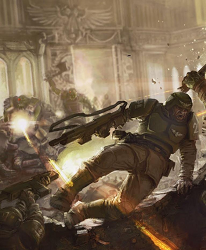
\includegraphics[width=\figwidth]{pics/5/19.png}
	\end{center}
\end{wrapfigure}
We were all locked, loaded, and ready for action when we entered the other team’s territory and the Interrogator made comm contact. 
She reported that the second team was pinned down in a building by several well armed cultists and hostile reinforcements were probably on the way. 
We would land on a nearby roof, get into position, then take out the attackers and any other cultists while the team inside finished their mission. 
The agents would stay in the flier and give air support if needed.

As soon as the flier touched down we fanned out across the edge of the roof and started setting up for one hell of a sneak attack. 
The targets below us were obviously professionals: 
they were spread across several pieces of cover, had military grade weaponry, and were maintaining fire discipline. 
Since these guys were head and shoulders above the cultists we had fought earlier, Sarge ordered us to hold fire and pick our targets for a massive opening salvo. 
Before any of us could finish setting up our shots though, the Interrogator ran to the edge of the roof and started pouring bolt fire onto the cultists below.

They responded instantly; 
every one of them turning towards the roof and laying down suppressive fire. 
We all immediately hit the deck, leaving the Interrogator as the only clear target.
She threw up a force shield, but she wasn’t a powerful offensive psyker and after a few seconds she collapsed with a scream.
When Nubby saw this he burst out of cover and started hosing las fire back at the cultists with no regard for his personal safety. 
Doc barely managed to pull him to the ground before their return fire killed him. 

Sarge took stock of the situation, decided it was salvageable, and assumed operational command. 
Figuring he needed some form of identification for when he reached the other team, he grabbed the moaning Interrogator’s bolt pistol with its obvious =][= marking, then ordered Twitch to take her back to the flier.

\begin{wrapfigure}{O}{\figwidth}
	\begin{center}
		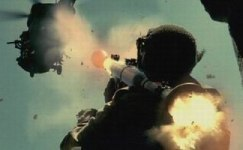
\includegraphics[width=\figwidth]{pics/5/20.png}
	\end{center}
\end{wrapfigure}
Twitch grumbled and pulled the limp Interrogator over his shoulder then started to slowly haul her towards the flier, complaining loudly that she wasn’t even trying to walk. 
Sarge decided that the squad’s current positions were fucked, so he gave the order to pop smokes and flashes then get into new ones. 
While we shifted positions, Sarge started flipping through frequencies on his combead in an attempt to contact the other team and coordinate an attack. 
We were still waiting for the smoke to clear and the fight to resume, when Cutter spotted the cultists’ reinforcements coming in on their own flier.

We’d been ready for something like this though; 
both Sarge and Nubby had brought heavy ordinance along. 
Nubby got his launcher ready, and as soon as the flier came into range he nailed it with a Flakk missile. 
The shot wasn’t perfect, and the pilot managed to make a crash landing at the edge of the smokescreen, but Sarge raised his nade launcher and dropped several rounds onto it before anyone could get out. 
That done with, he went back to scanning the comm channels and finally made contact with the other team. 
Sarge asked for a sitrep and we all got patched in just in time to hear “Our situation is FUBAR.  
We’re pinned down by several heavily armed cultists, and someone just fragged our Interrogator's flier.”

Whoops.

\begin{wrapfigure}{O}{\figwidth}
	\begin{center}
		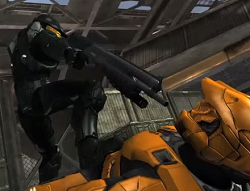
\includegraphics[width=\figwidth]{pics/5/21.png}
	\end{center}
\end{wrapfigure}
That was a little embarrassing, but these sort of things happen in combat and we were still in the middle of a fight. 

Sarge told them that we had eyes on the cultists and would deal with things while the other team sat tight. 
As the smoke cleared he started dropping nades onto every piece of heavy cover he could see while the rest of us waited for him to flush out the targets. 
A few seconds later the other team voxed back and told us to “Bloody hurry, cause they’re dropping nades right on our heads here.”

Double whoops.

This screw-up was too big to be ENTIRELY our fault. 
In fact there was no way that a screw-up this big could be accidental. 
After all, the Interrogator had been in comm contact with the other team the whole time and had been the first one to open fire...

We all turned our heads towards Twitch and the Interrogator and watched in horror as she sprang upright with Twitch’s laspistol in her hand. 
Twitch reacted with lightning speed and threw himself backwards, but before he hit the ground she drew a bead on his head. 
She met his eyes, and then, with the most beautiful smile in the entire galaxy, she pulled the trigger.

\begin{wrapfigure}{O}{\figwidth}
	\begin{center}
		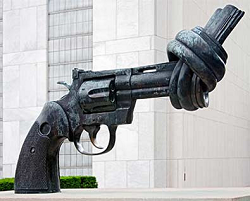
\includegraphics[width=\figwidth]{pics/5/22.png}
	\end{center}
\end{wrapfigure}
This was Twitch’s laspistol though; 
its owner was a man who once put directional charges on the backplate of his armor just to make sure no one snuck up behind him. 
There was an ominous hum when the trigger was depressed, the smile faded, and a second later the pistol’s power cell went off like a small grenade.
Taking the bitch’s hand with it.

It really shouldn’t have surprised any of us that Twitch had booby-trapped his weapons. He’d regularly told us to never, ever touch any of his stuff without asking first. 
It surprised us anyway though, and we all stared at the explosion like a bunch of dumb recruits. 
This meant that every one of us was dazzled by the explosion which blew Twitch and the Interrogator in opposite directions. 
As most of us tried to blink the spots out of our vision, Cutter charged for the downed Interrogator while swearing at the top of his lungs.

Cutter was damned fast, but he had a lot of distance to cover and the Interrogator was back on her feet in seconds. 
She sprinted for the flier and one of the agents poked his head out of the door to see what the hell was going on. 
What he saw was a badly wounded Interrogator running for safety while Twitch blindly sprayed las-fire and Cutter bore down on her revving his chainsword and screaming for blood, so in retrospect his decision to draw his sidearm and give her some covering fire was pretty reasonable. 
Reasonable or not it still screwed us though; Cutter had to start dodging shots and only caught up right as the Interrogator was boarding the flier.

Cutter made a good attempt at removing the Interrogator’s pretty head, but he was forced to dodge at the last second by the agent. 
The Interrogator’s counter stroke nearly impaled Cutter, but he fell back and only took a minor stab wound from her force sword. 
This gave the agent enough time to slam the door shut, and the flier started to take off as Cutter futilely hacked at the door with his chainsword.

\begin{wrapfigure}{O}{\figwidth}
	\begin{center}
		
\includegraphics[width=\figwidth]{pics/5/23.png}
	\end{center}
\end{wrapfigure}
The moment the Interrogator broke for the flier Sarge started trying to raise the agents on the comm, but to his absolute disgust he found that the Interrogator had locked the whole squad out of the team’s network. 
So with no way to get our side of the story across we just stood there and watched the flier take off. 
Our paralysis lasted until we realized that it was coming around for a strafing run. 

It didn’t surprise any of us that the agents had sided with their precious little Interrogator. 
Later on we might try to bring them around, but right then they were sheltering our enemy and trying to kill us. 
We all scattered and managed to avoid the first salvo from the flier’s nose gun.

Thinking fast, Doc grabbed the missile launcher from a stunned Nubby and loaded our backup Flakk round. 
Doc wasn’t exactly a pro at using the heavy weapon, but it was a pretty near miss and he definitely got a chunk of the flier. 
Sarge supplemented this with some airburst grenades from his launcher, and between the two of them we convinced the flier that we weren’t worth the trouble. 
It turned tail and limped away into the distance as we all stood there and tried to figure out what the hell just happened.

We were brought back to reality by the sound of fighting from the street below. 
The cultists in the building were laying heavy fire onto the poor buggers that we’d done our level best to teamkill. 
Doc went to see to the slightly crispy Twitch and slightly stabbed Cutter, while Sarge and Nubby pumped the rest of the squad’s grenade and missile launcher rounds into the building. 
This went a long ways towards convincing the other team that our previous attacks had all been a misunderstanding.

The barrage of explosives pretty much leveled the building, and none of the surviving cultists decided to stay and fight. 
Neither our squad or the team below was in position to give chase, so we all withdrew and tried our best to sort everything out over the comm.

\begin{wrapfigure}{O}{\figwidth}
	\begin{center}
		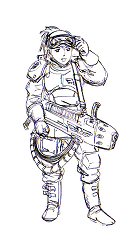
\includegraphics[width=\figwidth]{pics/5/24.png}
	\end{center}
\end{wrapfigure}
We explained the situation as best we could, and, mostly thanks to the former guardswoman on their team, we eventually convinced them that this was all our Interrogator’s fault. 
The problem was that we didn’t really have any idea what to do about it.
We were just a bunch of grunts, and the other team was down to a guardswoman, a psyker, an arbite, and a pair of badly wounded clerics. 
Apparently the Interrogator and all of their team’s nerds had been on the flier that Sarge and Nubby had blown to pieces. We blamed that one on the agents in the flier when they asked who had shot it down.

None of us had any great ideas about how to track down the Interrogator, so we decided to fall back to the other team’s safehouse and see if we could raise the third team’s Interrogator. 
We hotwired a pair of vans, and as we headed for their base Doc did his best to fix up the two wounded clerics. 
Neither of them was going to be back in the fight anytime soon though. 

On the brighter side, Twitch had lost his eyebrows and needed a new pair of pants, but was otherwise fine. 
And Cutter hadn’t even noticed the shallow stab wound he took, as he was far more concerned about the teeth his chainsword had lost when he tried to cut open the flier. 
The rest of the squad was completely unharmed, but Nubby was deeply depressed over the Interrogator’s treachery. 
We tried to be understanding, but it was hard. Especially when he started spinning theories about what could have FORCED her into betraying us all.

When we got to the safehouse we all went about reloading and rearming ourselves while Sarge and the Guardswoman tried to contact the third team. 
Luckily there was a backup flier parked at the safehouse, so we started moving everything we might need into it in case the third Interrogator wanted us to join him. 
After only a few minutes of this we started to hear the distinctive sounds of heavy artillery and las fire in the distance.

\begin{wrapfigure}{O}{\figwidth}
	\begin{center}
		
\includegraphics[width=\figwidth]{pics/5/25.png}
	\end{center}
\end{wrapfigure}
We quickly realized that our Interrogator had called in another purge for Emperor knows what reason. 
Being inside an inexorably shrinking military cordon is bad, so we decided it was time to get the hell out of dodge. 
We loaded up the wounded and the last of the supplies we could carry, then the Arbite got us into the air while Sarge and the Guardswoman tried to use the flier’s vox to reach the local authorities.

We were wildly unsuccessful in our attempts to convince the PDF to stop the purge. 
Their orders had been given by someone with a genuine Inquisitorial Rosette, and Emperor help the man who defies the Inquisition. 
Sarge failed miserably when he tried to explain that WE were the Inquisition, as without a Rosette to prove it no one would believe him. 
We considered going back to look for the second team’s Rosette, but since their Interrogator had been wearing it when we blew him to pieces that idea was quickly abandoned. 
Eventually the PDF must have reported our attempts to stop the purge to the Interrogator, because they suddenly got very interested in where we were voxing them from. 
We quickly deactivated our vox, in case they could trace it, and watched the fireworks below us while we made our way towards the third team’s last known position.

We spent a lot of time talking during the flight, none of this shit made any sense to us and we had no idea what to do about it. 
Initially we asked Twitch what the Interrogator’s plan was since he’d been sure she was planning to kill us the entire time, but he quickly devolved into theories about “precious bodily fluids.” 
Nubby wasn’t any help either; 
he kept insisting that this was all some sort of misunderstanding and the Interrogator was a sweet girl who would never hurt a fly. 
We weren’t going to get anything useful out of them, so we put our heads together with the rest of the team and tried to figure shit out.

\begin{wrapfigure}{O}{\figwidth}
	\begin{center}
		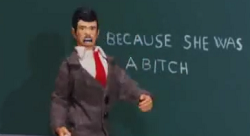
\includegraphics[width=\figwidth]{pics/5/26.png}
	\end{center}
\end{wrapfigure}
Looking back it was sort of weird that the cultists at the party hadn’t been genestealery or cared about shooting the fat man, so we decided that they must have been the Interrogator’s friends and the plan had been to wipe out the whole team. 
If that was her main goal though she could have killed us all in far simpler ways, so we figured that it was supposed to look like an accident. 
We didn’t really see the point though. 
If she just wanted to order purges it provided a nice justification, but she hadn’t ordered a general purge on the first cult. 
Maybe she wanted to perpetrate a mass murder and still pass her Inquisitor Test or something.

Anyway, it was definitely her plan to get us into a fight with the other team and presumably have us wipe each other out. 
We didn’t really see a reason for that either, but maybe she just wanted to kill the other team and figured she’d take out two birds with one stone. 
It made a stupid sort of sense if she was low on cultist manpower and afraid of people trying to stop her purges. 
Her reason for the purges was still a mystery though; 
all we knew was that that she wasn’t working with the genestealers, since they weren’t going to live through the purges either. 
In the end we decided that she was just an utter bitch and tried to catch what sleep we could before the flight ended. 

We woke to the sound of more artillery fire. 
We were over the city where the last team was supposed to be working, and we all recognized the shitstorm below us. 
The damned bitch had ordered another purge. 
We were pretty sure she couldn’t have ordered this one without either enlisting or killing the third Interrogator, but it didn’t hurt to check. 
We turned the vox back on called the third team, and to our surprise we actually got them on the first try.

Sarge immediately explained that our Interrogator had gone nuts, tried to get us to kill the other team, and was running around ordering mass purges for generic evil reasons.

\begin{wrapfigure}{O}{\figwidth}
	\begin{center}
		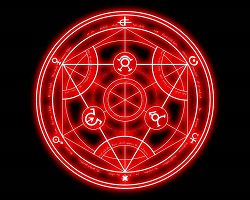
\includegraphics[width=\figwidth]{pics/5/27.png}
	\end{center}
\end{wrapfigure}
Unfortunately the Bitch had their Interrogator under her thumb, so the only response we got was an order to surrender to the Inquisition and seek mercy for our sins. 
That was bullshit so we turned the vox back off and started to debate the merits of catching a ride back to Oak’s ship, hanging out on some tropical island until this all blew over, or even getting a job on a rogue trader. 
Our boss was an evil bitch who got off on ordering mass purges, the nearest other official was totally whipped by said evil bitch, several major cities were being needlessly genocided, and no one on this damned planet would listen to us unless we had one of their Rosettes. 
Everything was a horrible bloody mess and it shouldn’t have been our job to sort it out.

Our plans for desertion came to a sudden halt when the pysker from the second team started freaking out. 
We hadn’t known this psyker for very long, but he didn’t seem like the type to randomly start screaming; 
so while Doc saw to him we all started looking out the windows and checking the sensors for anything warpy going on. The problem quickly became apparent:
 a pair of massive glowing lines shot in different directions across the ground under us. 
A second later this was followed by dozens of smaller lines which formed eldritch symbols all across the city below.

We weren’t exactly geniuses, but it didn’t take a bloody savant to see that this was some serious warp shit or that the two glowing lines were extending towards the other two cities that the Interrogator had ordered purged. 
Even though none of us were sure about what was going on here, everyone was pretty sure this was all her fault. 

The situation was going to shit at incredible speed. 
The only thing we could think to do was to try and get our hands on one of the two remaining Rosettes and use it to tell everyone to stop being retarded. 
So we stayed on course for the third team’s base and hoped that both Interrogators would still be there.

\begin{wrapfigure}{O}{\figwidth}
	\begin{center}
		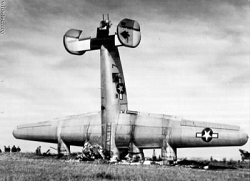
\includegraphics[width=\figwidth]{pics/5/28.png}
	\end{center}
\end{wrapfigure}
While we flew everyone geared up for a fight; 
we weren’t going to ask nicely and appeal to reason then be really surprised when they all sided with the hot chick over a bunch of scruffy guardsmen. 
We were going to hit them hard and let the Emperor sort them out. 
After this shit was over we could argue with any survivors while Doc tried to reattach their limbs.

We sold the remnants of the second team on our plan. 
The Guardswoman and the whimpering psyker would come with us while the arbite handled the flier and kept an eye on with the two wounded clerics still chilling in the back. 
The plan was pretty simple: bust in, head for the two Interrogators, kill or subdue anyone in the way, and hopefully grab one of those damned Rosettes intact. 
It was going to be a tight and brutal fight; 
several well trained hostiles, a lot of walls of varying thickness, an enemy who knew the terrain better than us, severe consequences for failure, and to top it off it looked like the safe house was located halfway up a damned tower. 
Not only would it be a rough fight, we also had to figure out a way to get inside without running into an ambush. 
Good thing we had a flier.

Now, this flier didn’t have any weapons, so we couldn’t really use it for air support. 
It did have a nice amount of armor though, and the third team’s safehouse had some nice big windows…

A few minutes later we finally forced open the flier’s doors and started digging our way out of the pile of safety glass, wall fragments, and destroyed furniture we had created with our landing.

\begin{wrapfigure}{O}{\figwidth}
	\begin{center}
		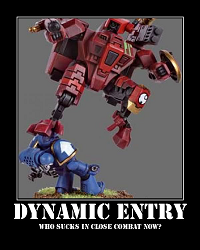
\includegraphics[width=\figwidth]{pics/5/29.png}
	\end{center}
\end{wrapfigure}
All things considered, it was incredibly lucky that we were the first ones out of the wreckage. 

As we stumbled out of the crippled flier we saw several hostiles struggling to get free, and we took the chance to hit them with some of Doc’s, now normal strength, tranqs. 
We congratulated ourselves on successfully breaching the perimeter without even killing any other Inquisitorial agents. 
Probably. Truly we were the pinnacle of professionalism.

After we finished patting ourselves on the back over our dynamic entry we formed up and started making our way deeper into the safehouse. 
We knew how to clear a building and had plenty of flash grenades, so we moved from room to room at a steady pace, flashing, sweeping, and securing. 
The first few rooms were all empty, but before long we ran into a pair of adepts who practically shit themselves when we flashed them. 
We clubbed them down, secured their hands and feet, and then asked them a few questions about where exactly everyone was.

The adepts were actually very helpful. 
They made a few feeble attempts to defy us, but after Sarge hauled them both to a window and pointed out the glowing shit both adepts came around to our way of thinking. 
They also found Cutter’s explanation of how the Three Strikes rule works with a chainsword very persuasive. 
They pointed us towards a set of rooms that belonged to the third team’s Interrogator and confirmed that our former Interrogator was in there with him. 
We taped them to the wall and made our way towards the Interrogators; 
there was going to be a reckoning.

\begin{wrapfigure}{O}{\figwidth}
	\begin{center}
		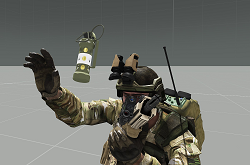
\includegraphics[width=\figwidth]{pics/5/30.png}
	\end{center}
\end{wrapfigure}
There are two good ways to clear a hostile building. 
You either want to hit hard and fast with several teams working together to take out the enemy before they concentrate their forces, or you want to move in stealthily and take out small groups of enemies while avoiding major ones. 
Unfortunately the small size of our team and our arrival via a crashing flier meant that these good options weren’t really possible. 
We were stuck with the sorta-almost-ok option of just moving carefully and praying to the Emperor that we’d spot the inevitable ambush before it was sprung. 
We didn’t.

We methodically worked our way towards the room where the Interrogators were supposed to be; 
we had it down to a science. Every room went the same: 
check the door, get into position, flash, storm, realize the room was empty, and move on to the next door. 
The lack of opposition was unsettling, and we were all on pins and needles when we got to a door that was sturdier than any of the others we’d seen. 
If the adepts had been telling the truth, both the Interrogators were inside.

We got into position and readied our weapons while Twitch checked the door for traps and quietly unlocked it. 
Sarge got a firm grip on the handle, cooked a flash, cracked the door open, and tossed it through. 
Before he even started to close the door the grenade bounced off something in mid air and sailed right back through. 
Sarge managed to get out an “OH SHI-” before the flash went off about eight inches in front of his face.

\begin{wrapfigure}{O}{\figwidth}
	\begin{center}
		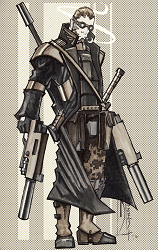
\includegraphics[width=\figwidth]{pics/5/31.png}
	\end{center}
\end{wrapfigure}
Sarge’s shout triggered the bone deep reflexes that all guardsmen develop, and the rest of us managed to turn away. 
Everyone was still dazzled and deafened, but at least we weren’t completely blind. 
Also, our turn meant that we just happened to be looking in the right direction when the two agents dropped in through the ceiling. 
They landed on our flanks in perfect crossfire positions, and even though we were all deafened we could FEEL heavy boots pounding towards the door. Thank the Emperor that one of the agents came down next to Twitch and Cutter.

The agent who came down next to Twitch and Cutter was the social one we had gone through such trouble to rescue back at the party, and as he landed he raised a pair of autopistols. 
He had about a quarter second to look surprised before a full auto burst hit him in the chest and a chainsword hit him in the neck. 
That taught him to be ungrateful to his rescuers.

The second agent landed next to the guardswoman and psyker, neither of whom had reaction times as good as Twitch and Cutter. 
Before the guardswoman managed to raise her lasgun the agent landed a brutal kick on her head, raised his autogun, and opened fire on the the psyker and Nubby. 
The poor bastard didn’t have a chance to do anything, but his death gave Nubby the split second he needed. 
With weasley speed Nubby got behind the collapsing psyker and held him up like a shield while he sprayed the agent with wild las-fire. 
The Emperor was with Nubby: 
several of the unaimed shots hit the agent and Doc’s followup salvo finished the job.

The entire fight had taken just a few seconds and the smoke from the flash was still fading as the second agent crumpled to the ground. 
The psyker was dead, the guardswoman was groggily cursing the dead agent, a barely conscious Sarge was lying on the floor, but the rest of us were okay. 
We had about two seconds to take stock of the situation before the the door burst off its hinges and landed squarely on Sarge.

\begin{wrapfigure}{O}{\figwidth}
	\begin{center}
		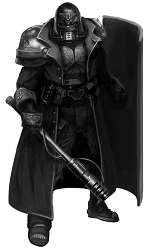
\includegraphics[width=\figwidth]{pics/5/32.png}
	\end{center}
\end{wrapfigure}
The door was followed by a pair of heavily armored arbites carrying shields and shock mauls. 
Shields raised, they stood right on top of door and looked really confused when they saw an entire squad of guardsmen facing them with weapons raised. 
There was a brief pause while the arbites realized that the agents were already dead, and we all stared at the feebly cursing lump being crushed under a heavy door and three hundred kilos of arbites. 
Then Cutter ran in with a scream and the fight was on.

Cutter did most of the work this time; there’s just no good way to use a suppression shield to stop both las-fire and a maniac with a chainsword. 
The arbite on the left made a decent attempt at it though: 
he held off several strikes from Cutter and shots from Twitch and Doc while his buddy kept Nubby and the guardswoman from shooting him in the back. 
He couldn’t keep it up though. 
A thrust from Cutter’s sword nearly made it through, and the arbite parried the strike right into his buddy’s back.

The wounded arbite staggered forward and removed over a hundred kilos of meat and armor from Sarge’s back. 
With a roar of rage Sarge pushed himself upward and managed to unbalance the arbite that was still on top of him. 
We all seized the opportunity and several volleys of las-fire got past the arbites’ shields, ending the fight.

While the rest of us restrained the badly wounded arbites and hauled them out of the way Sarge slowly pushed himself off the floor. 
With a pained groan he got his feet under him and lifted the reinforced door, complaining about its weight and cursing arbites in general as he did so. 
Right as Sarge managed to get upright, his curses were interrupted. 
A pair of bolt rounds came through the doorway and slammed into the remains of the door and his back.

\begin{wrapfigure}{O}{\figwidth}
	\begin{center}
		
\includegraphics[width=\figwidth]{pics/5/33.png}
	\end{center}
\end{wrapfigure}
The door took the brunt of the damage, but Sarge was thrown forwards and slammed into the wall head-first. 
This was the final straw, and Sarge slipped into unconsciousness as Doc hastily grabbed him and dragged him out of the line of fire. 
From inside the room we heard the third team’s Interrogator yell at us to surrender in the name of the Holy Inquisition. 
A quick peek revealed that both he and the Bitch were holed up behind a makeshift barricade and had bolt pistols trained on the door.

So no shit, there we were, standing outside a room containing a pair of hostile and well armed Interrogators manning a prepared position, and with no noncom to tell us what to do. 
Up to now we had always looked to Sarge when the going got tough, but he was out for the count. 
Twitch and Nubby immediately started arguing with each other, Cutter sat on one of the wounded arbites and worked on dislodging a piece of armor from his chainsword, Doc got Sarge comfortable in a corner, and the guardswoman stared at us like we were a bunch of retards. 

Eventually Doc got tired of the guardswoman giving him the stinkeye and decided that it was his duty as the only sane member of the squad to take charge. 
He put down his medkit, hefted his lasgun, crept as close to the doorway as was safe, and politely asked the third team’s Interrogator if he’d consider surrendering the Bitch to us.

This resulted in a brief astonished silence and several bolt rounds sailing through the open doorway.

\begin{wrapfigure}{O}{\figwidth}
	\begin{center}
		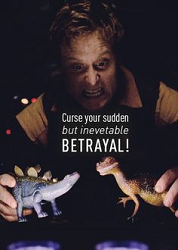
\includegraphics[width=\figwidth]{pics/5/34.png}
	\end{center}
\end{wrapfigure}
Doc was not deterred though. 
As the rest of the squad watched in disbelief he repeatedly tried to convince the two Interrogators to stand down. 
It really was something to see: 
Doc standing against the wall and calmly laying out our grievances and arguing Inquisitorial regulations. 
Especially considering that they would periodically fire bolt rounds at him. 
The crazy part was that he actually seemed to be making progress: the more he argued the more thoughtful the third team’s Interrogator sounded and the more furious the Bitch sounded. 
The tipping point was when the guardswoman chimed in, confirmed Doc’s story, and asked the Interrogator to look out the window at the glowing warpy stuff.

We heard him get up, walk to the window, and exclaim about it being a “three-fold sacrificial ritual.”
A second later we heard the distinctive sound of the Bitch’s force sword, a meaty thunk, and the most sulfurous swearing to ever come out of such a beautiful mouth. 
The good news was that there was just one hostile Interrogator now.

\begin{wrapfigure}{O}{\figwidth}
	\begin{center}
		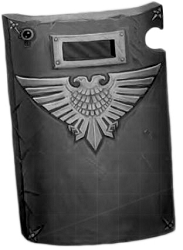
\includegraphics[width=\figwidth]{pics/5/35.png}
	\end{center}
\end{wrapfigure}
Diplomacy wasn’t going to work this time, though Nubby made a few attempts which only resulted in more swearing and bolt-fire. 
We wanted to just rush her, but our former Interrogator was a damned good markswoman and none of us were keen to try trading shots with her. 
We started trying other things: like grenades and blasting holes in the walls. 
Unfortunately we quickly discovered that the walls were too sturdy to blast through without collapsing the building, and she bounced every grenade back with her damned telekinesis. 
The best we could do was pop a smoke on our position and hope it wafted towards her.

We were running out of options that wouldn’t result in one of us getting shot when Doc remembered the arbites’ shields. 
Two of us could charge in under smoke cover then try to flank her while the rest of the squad gave suppressing fire from the door. 
Hopefully the shields would hold long enough to get close to her and allow the rest of the team a chance to move forward. 
Cutter was an obvious choice for rushing in, but it surprised the hell out of us when Nubby volunteered to carry the other shield.

This behavior was very suspicious coming from Nubby. We reminded him that the Interrogator was a heretical super-bitch, but he just wouldn’t listen. 
He insisted that she was a nice girl who just got stuck “runnin’ wif a bad crowd.” 
We pointed out that she tried to kill us all, he said that most of our superior officer had too. 
We pointed out that she had killed the other Interrogator, he said that we’d been planning to do that too so we shouldn’t judge her for it. 
Finally Doc pointed out the she had stabbed Cutter and would stab Nubby too if she got the chance. 
Nubby maintained that “lotsa people ‘ave stabbed Cutter, I’m not worried, I fink she likes me deep down.” 

We gave up at this point and just gave him the damned shield. With any luck Cutter would get to her first and chop her head off before Nubby had a chance to be retarded.

\begin{wrapfigure}{O}{\figwidth}
	\begin{center}
		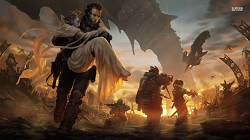
\includegraphics[width=\figwidth]{pics/5/36.png}
	\end{center}
\end{wrapfigure}
We got ready, popped the smoke, and Nubby and Cutter ran towards opposite sides of the room. 
Cutter was faster by far, but right as he got close the Interrogator landed a grenade at his feet while staggering him with bolt rounds. 
Cutter leapt backwards in time but the blast still sent him and his shield flying across the room, Nubby took advantage of the distraction though. 
We all heard a clang as he clubbed the bolt pistol out of her hands, and another as he knocked her to the ground.

The rest of us started moving forwards, but stopped in sheer shock when we heard the Interrogator surrender to Nubby. 
She admitted that she had been forced to work against the Imperium by evil heretics who would kill her if she disobeyed. 
She just wanted to be safe.

We cleared the smoke and watched in amazement as he reached down and helped her up, quietly telling her that he’d make sure it all worked out as he did so. 
He’d protect her from the “bad people,” no one would ever hurt her again. 
Then in a fluid movement she drew her force sword, swung it in a circle, and bolted for large security door at the far end of the room as Nubby fell to the ground screaming.

\begin{wrapfigure}{O}{\figwidth}
	\begin{center}
		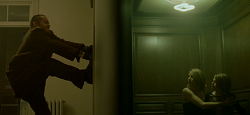
\includegraphics[width=\figwidth]{pics/5/37.png}
	\end{center}
\end{wrapfigure}
Twitch and the guardswoman opened fire on her as she ran, but her damned shield held out just long enough for her to pass through the door and lock it behind her. 
Doc ran over to Nubby and found him lying a full meter from his legs; 
it was a bad wound but the cut had been across the thighs not the belly. 
Thinking fast, Doc put a tourniquet on both legs and started a blood transfusion. 
While he worked he lectured Nubby about the importance of critical thinking and listening to other peoples’ advice.

Twitch, the guardswoman, and a moderately wounded Cutter walked over to the security door to see if they could get through it. 
To their surprise it wasn’t an escape passage, it was a panic room. 
A little fiddling got the comm-screen working, and they were treated to the sight of a furious Interrogator sitting in the middle of a small rune covered room with a bloody sword in hand. 
A bit more poking let them find the transmit switch and Twitch formally placed the Interrogator under arrest and ordered her to turn over her Rosette and any bodily fluids she had stolen. 
She burst into hysterical laughter at this.

To everyone’s surprise the Interrogator actually started monologuing once she had finished laughing. 
Her defeat by a band of dubiously competent guardsmen had apparently unhinged her.  
Her brethren had spent years preparing this ritual, the blood of innocents slain by their very protectors would fuel a warp-storm which would tear this entire blah blah blah, I’m a heretical-super-bitch, blah blah. 
When she started ranting about the glory of Chaos Twitch, Cutter, and the guardswoman quickly became bored and walked away from the intercom; 
leaving the infuriated Interrogator shouting about being able to watch us all die to the horrors of the warp before they claimed her.

While the guardswoman went to help Doc and Cutter guarded the security door, Twitch wandered over to the headless Interrogator. 
He poked the dead man with his lasgun, in the official Guard method for determining the icky-ness of a corpse, then grudgingly started going through the man’s pockets when the guardswoman shouted at him to stop being a pansy. 
Twitch found the Rosette pinned to the Interrogator’s high collar. 
Well, most of it: the top quarter of the little device was feebly sparking in the puddle of blood spreading from the severed head. 
Twitch got out his roll of duct-tape and went to work, but the end result didn’t look very Inquisitorial. 
Also the data-jack was full of... fluids.

\begin{wrapfigure}{O}{\figwidth}
	\begin{center}
		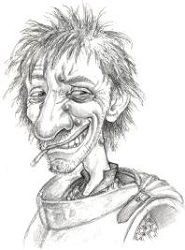
\includegraphics[width=\figwidth]{pics/5/38.png}
	\end{center}
\end{wrapfigure}
On the other side of the room Doc was finishing the field dressings and still giving Nubby shit. 
The subject had finally come around to how important it had been to get an Inquisitorial Rosette, and how Nubby had fucked it all up. 
Amazingly this got a response out of the semi-conscious Nubby.

> \todo{fix greentext}“Eh Doc, ‘choo remember how Sarge said I should stop goin’ fru peoples pockets? 
Well when I was helpin ‘er up, I started finken about ‘ow dat fancy bracelet of ‘ers was so ‘portant. 
I figured dat if she was all being bossed round by chaos an’ such, she prob’ly shouldn’ be ‘lowd to keep it. 
So I nicked it while she was busy cuttin’ me legs off”

And just like that we won. 
The little shit’s kleptomania had saved us all. 
After years of telling Nubby to stop stealing people’s stuff, he grabbed the one thing that really mattered.

He was still an idiot though.

Doc grabbed the Rosette off of Nubby, tossed it to the guardswoman, and told her to comm to the PDF as fast as possible. 
We had completely destroyed the third team’s comm systems, but the flier’s vox was still intact. 
The arbite and guardswoman started arguing with PDF officers and government officials from the wrecked cockpit. 
While they were trying to get the brass to see reason and stop feeding the giant sacrificial circle, seriously it was all glowing and shit, the rest of us decided what to do about the Interrogator.

She had really started freaking out when she realized the Rosette was missing, but the sight of Cutter chilling outside her door with his chainsword ready had convinced her to stay inside. 
We either needed to kill her or capture her; 
and as attractive as the first option was, it would be much easier to smooth things over with Oak if we were able to turn her over. 
The debate ended when Sarge pried himself up, staggered in, and ordered Twitch to weld the panic room shut.

\begin{wrapfigure}{O}{\figwidth}
	\begin{center}
		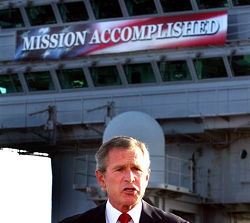
\includegraphics[width=\figwidth]{pics/5/39.png}
	\end{center}
\end{wrapfigure}
With Sarge bossing us around we started getting shit done again.

Twitch blast welded the panic room shut, Doc went to help convince the PDF to stop being retarded, and Cutter started dragging all the wounded together for triage. 
Sarge and Nubby just sort of hung out and basked in the sound of the Interrogator’s outrage.

As the purges were called off the giant glowy runes faded away and the Interrogator’s curses attained a whole new level of venom. 
That venom faded after Twitch found the panic room’s air intake and sealed it shut. 
We all sat around and watched as she slowly ran out of fresh air and passed out, then we waited a bit longer. 
When Doc finally decided that she was either comatose or too hypoxic to cause trouble we cut open the doors, dragged her out, tranqued her, and left her in Doc’s capable hands.

Sarge became the de facto Interrogator at this point. 
The second team had been reduced to two functional members, and what remained of the third team was being restrained by a few dozen rolls of duct tape until the situation could be explained to them. 
A flier was requisitioned and Sarge took the guardswoman and arbite to go sort everything out with the local authorities while everyone else stayed in the wrecked tower.

The situation was explained in broad terms. 
A cordon was to be put around all three cities and the surgical strikes in the sealed orders were carried out, but no more mass purges would be done until a fully certified Inquisitor ordered it. 
Sarge told all the brass and bigwigs to just sit tight and wait for the guard regiment to arrive with their senior Inquisitor; 
they’d be able to sort out the chaos rune bullshit and decide whether the genestealer cults warranted a full purge.

\begin{wrapfigure}{O}{\figwidth}
	\begin{center}
		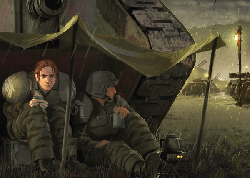
\includegraphics[width=\figwidth]{pics/5/40.png}
	\end{center}
\end{wrapfigure}
We used the Rosette to requisition a ride from the navy. 
We made sure everything was sort of stable before we left, but as far as we were concerned our mission now consisted of getting the Interrogator back to Oak as soon as possible.

The guardswoman who had helped us through the last battle decided to stay with the arbite, the two wounded clerics, and the rest of the third team. 
The local authorities needed the help of some people who knew how genestealers worked while they waited for the Inquisitor to show up. 
After Sarge had requisitioned our ride home and convinced the navy we were serious people he handed the Rosette over to her; 
hopefully she would keep things from going all to shit before help arrived. 
As a sort of afterthought we formally invited her to hang with our regiment if she ever got back to base.

That done with we packed up our gear, wounded dumbass, and sedated Interrogator; 
then we got the hell off the planet.

\begin{wrapfigure}{O}{\figwidth}
	\begin{center}
		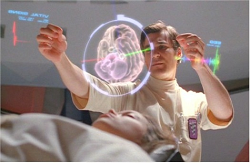
\includegraphics[width=\figwidth]{pics/5/41.png}
	\end{center}
\end{wrapfigure}
Sedating a person for a long period of time doesn’t really work. They tend to spontaneously die or just not wake up. 
This isn’t an issue if you have a stasis pod, but that’s not something you can get on most Imperial frigates so we had to improvise a little bit.

Letting the Interrogator sit in a cell was an invitation to disaster: 
it wouldn’t be a day before she convinced some swabby to let her out, so we went the cold hearted medical route. 
Doc brushed up on his reading, got the senior ship’s surgeon to lend him a hand, in this case hand means doing most of the procedure for him, and installed a shunt in the Interrogator’s spine. 
This more or less paralyzed her from the nose down, and combined with a psychic damper it kept her from causing trouble.

She was kept in our private medbay next to Nubby. 
The force sword had done something nasty to Nubby’s legs, it was going to take augmetic surgery to get them back, but he was remarkably cheerful about the whole thing. 
He spent most of the journey talking to the Interrogator and telling her stories of our adventures. Keeping her spirits up and all that. 
He thoroughly enjoyed having someone to talk to who didn’t tell him to shut up or stop lying.

Doc taught the Interrogator how to communicate via blinking as a sort of experiment during the trip, but all she ever said was “kill me.” 
Nubby thought this was needlessly grim and redoubled his efforts to cheer her up.

\begin{wrapfigure}{O}{\figwidth}
	\begin{center}
		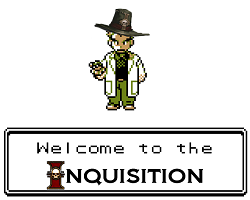
\includegraphics[width=\figwidth]{pics/5/42.png}
	\end{center}
\end{wrapfigure}
When we finally got back to Oak’s spacefaring Inquisitorial school, Sarge handed over a report of the squad’s adventures and refused to budge until a senior Interrogator confirmed that the report had been read and collected the Interrogator. 
Nubby was sad to see her go, and hoped that she would come visit after the Inquisition helped her with the “bad men.”

We were all released to our quarters on Oak’s ship; except for Nubby who got sent to the medical wing to start getting fitted for a pair of augmetic legs. 
We were finally able to relax in the company of our fellow guardsmen, but we weren’t able to get into the proper spirit of R\&R (see: Drunk) since we knew that Oak would call us up for a debriefing the moment we started drinking. 
He didn’t keep us waiting long though: before the week was over we were summoned to his office to give a full report.

Sarge and Doc did their best to explain everything while Twitch and Cutter kept their damned mouths shut, and to our surprise Oak believed every word. 
He questioned a few things and asked for clarification several times, but he believed every bloody word we said. 
At the end of the debriefing he told us the Interrogator was being turned over to the Ordos Malleus for interrogation, and we were never to speak of her again. 
This suited us fine and we all started congratulating ourselves on a job well done, then he offered Sarge the rank of Interrogator and a chance to advance to full Inquisitor.

\begin{wrapfigure}{O}{\figwidth}
	\begin{center}
		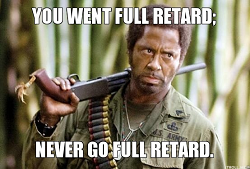
\includegraphics[width=\figwidth]{pics/5/43.png}
	\end{center}
\end{wrapfigure}
The entire squad went to bat for Sarge when we heard this.

Cutter expressed his lack of faith in Sarge’s combat ability. Twitch pointed out his lack of proper Inquisitorial suspicion. 
Doc raised the question of Sarge’s overall physical fitness and mental fortitude, and from his comm link in the medbay Nubby raised the question of Sarge’s lack of ethics and history of petty theft. 
None of us could condone the elevation of such a pitiful specimen to the rank of Interrogator. 
It would dishonor the entire Inquisition. In the face of all these perfectly valid arguments Sarge regretfully declined Oak’s offer; 
he just wasn’t good enough to be an Interrogator, so he’d have to settle for being a simple sergeant.

A very bemused Oak acquiesced to Sarge’s rejection, if the man’s best friends didn’t think he was interrogator material that was the end of it. 
So he finished the debriefing and sent us on our way.
We went and drank until we puked, and then puked until we passed out.
Except for Nubby, he was stuck in medbay eating and drinking nothing but nutritionally balanced meals, poor little bugger.

\begin{wrapfigure}{O}{\figwidth}
	\begin{center}
		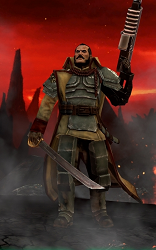
\includegraphics[width=\figwidth]{pics/5/44.png}
	\end{center}
\end{wrapfigure}
Our R\&R binge lasted for quite a while, but eventually it came to an end. 
We geared up for our next mission, but unfortunately Nubby was still struggling with his augmetic legs. 
Learning to walk on artificial legs is a long and arduous process which not everyone can master, but Nubby had faith and assured us that he’d keep at it while we went on out next mission. 
Luckily, there was an open post in the quartermaster’s department on the ship. 
It would be the perfect job for him while he got his feet under him as it were.

We left the medbay after that discussion with heavy hearts. 
None of us had exactly *liked* Nubby, but we couldn’t imagine deploying without him. 
Where the hell would we get our ammo from? He always just seemed to have fresh packs for us.

As we got back to our barracks we were greeted by a familiar voice. 
Sitting in the middle of the room was the Rupert, complete with a shiny augmetic arm and Alfred at his back. 
He was chatting with Crisp, one of the few surviving flamer experts in the regiment, and seemed to be enjoying himself immensely.

In a jolly voice he invited us over and told us he wanted our help on a “Little trip down to the colonies to sort out a spot of theological trouble.” 
According to him it was, “Positively benighted down there not a single illuminated thinker on the whole planet, no one to point them towards the light of the Emperor. 
You might call it a case of Dark Heresy, wot wot?”

We gathered up our kits and followed him out. 
After all, we knew there were worse Interrogators out there…

